\documentclass{beamer}

\usepackage{beamerthemesplit}
\usepackage{graphicx}
\usepackage{subfigure}
\usepackage{amsmath,amssymb}
\usepackage{multimedia}
\usepackage{times}
\usepackage{calc}
\usepackage{array}
\usepackage{tabularx}


\usepackage[latin1]{inputenc}
\usepackage[T1]{fontenc}
\usepackage{listings}
\usepackage{courier}
\usepackage{color}

\newcommand{\re}{\text{Re}}
\newcommand{\im}{\text{Im}}
\newcommand{\de}{\mbox{d}}
\newcommand{\eref}[1]{(\ref{#1})}
\newcommand{\ii}{\text{i}}
\newcommand{\ee}{\text{e}}
\newcommand{\mathbi}[1]{\textbf{\em #1}}
\newcommand{\rem}[1]{}


% Layout specification

% \usetheme{AnnArbor}
% \usetheme{Antibes}
% \usetheme{Bergen}
% \usetheme{Berkeley}
% \usetheme{Berlin}
% \usetheme{Boadilla}
% \usetheme{boxes}
% \usetheme{CambridgeUS}
% \usetheme{Copenhagen}
% \usetheme{Darmstadt}
% \usetheme{default}
% \usetheme{Dresden}
% \usetheme{Frankfurt}
% \usetheme{Goettingen}
% \usetheme{Hannover}
% \usetheme{Ilmenau}
% \usetheme{JuanLesPins}
% \usetheme{Luebeck}
% \usetheme{Madrid}
% \usetheme{Malmoe}
% \usetheme{Marburg}
% \usetheme{Montpellier}
% \usetheme{PaloAlto}
% \usetheme{Pittsburgh}
% \usetheme{Rochester}
% \usetheme{Singapore}
% \usetheme{Szeged}
\usetheme{Warsaw}

% \usecolortheme{albatross}
% \usecolortheme{beaver}
% \usecolortheme{beetle}
% \usecolortheme{crane}
% \usecolortheme{default}
% \usecolortheme{dolphin}
% \usecolortheme{dove}
% \usecolortheme{fly}
% \usecolortheme{lily}
% \usecolortheme{orchid}
% \usecolortheme{rose}
% \usecolortheme{seagull}
% \usecolortheme{seahorse}
% \usecolortheme{sidebartab}
% \usecolortheme{structure}
% \usecolortheme{whale}
% \usecolortheme{wolverine}

% \usefonttheme{default}
% \usefonttheme{professionalfonts}
% \usefonttheme{serif}
% \usefonttheme{structurebold}
% \usefonttheme{structureitalicserif}
% \usefonttheme{structuresmallcapsserif}

% \useinnertheme{circles}
% \useinnertheme{default}
% \useinnertheme{inmargin}
% \useinnertheme{rectangles}
% \useinnertheme{rounded}

% \useoutertheme{default}
% \useoutertheme{infolines}
% \useoutertheme{miniframes}
% \useoutertheme{shadow}
% \useoutertheme{sidebar}
% \useoutertheme{smoothbars}
% \useoutertheme{smoothtree}
% \useoutertheme{split}
% \useoutertheme{tree}



% Meta

\title[odeint]{The Taylor series method for ordinary differential equations}
%\subtitle[odeint]{}
\author[Karsten Ahnert]{Karsten Ahnert$^{1,2}$ \\ Mario Mulansky$^{2}$}
\institute[Universit\"at Potsdam]{$^1$ Ambrosys GmbH, Potsdam\\ $^2$ Institut f\"ur Physik und Astronomie, Universit\"at Potsdam}
\date{December, 8, 2011}
\titlegraphic{\includegraphics[width=4cm]{ambrosys}\hspace{5ex}
\includegraphics[width=1.5cm,height=1.5cm]{logo}}
\subject{Subject}
\keywords{Keyword1,Keyword2}



\definecolor{dark-gray}{gray}{0.15}
\definecolor{light-gray}{gray}{0.8}
\definecolor{lighter-gray}{gray}{0.9}

\definecolor{dark-green}{rgb}{0,0.4,0}
\definecolor{dark-red}{rgb}{0.2,0,0}



\lstset{
         basicstyle=\tiny\ttfamily, % Standardschrift
         %numbers=left,               % Ort der Zeilennummern
         numberstyle=\tiny,          % Stil der Zeilennummern
         %stepnumber=2,               % Abstand zwischen den Zeilennummern
         numbersep=5pt,              % Abstand der Nummern zum Text
         tabsize=2,                  % Groesse von Tabs
         extendedchars=true,         %
         breaklines=true,            % Zeilen werden Umgebrochen
         frame=single,         
         backgroundcolor=\color{lighter-gray},
         tabsize=4,
         keywordstyle=\color{dark-green},
         identifierstyle=,
         commentstyle=\color{dark-gray}\normalfont\rmfamily\itshape,
         stringstyle=\color{dark-red},
         showspaces=false,           % Leerzeichen anzeigen ?
         showtabs=false,             % Tabs anzeigen ?
         xleftmargin=17pt,
         xrightmargin=10pt,
         framexleftmargin=17pt,
         framexrightmargin=5pt,
         framexbottommargin=4pt,
         language=c++,
         showstringspaces=false      % Leerzeichen in Strings anzeigen ?        
 }
\lstloadlanguages{C++}




% What is shown

\beamertemplatenavigationsymbolsempty
\setbeamertemplate{footline}{}
\setbeamertemplate{footline}{\insertframenumber}
\setbeamertemplate{headline}{}


\parindent0pt











\begin{document}



\frame{
  \titlepage


}

\frame{
  \frametitle{Outline}
  \tableofcontents
}

\section{Solving ODEs}

\begin{frame}[fragile]{Solving Ordinary differential equations numerically}

    Find a numerical solution of the initial value problem for an ODE
    \[ \dot{x} = f(x,t) \,\,\textrm{,} \quad \quad x(t=0) = x_0\]

   \vspace{2ex}

   Example: Explicit Euler
   \[ x(t + \Delta t ) = x(t) + \Delta t \,\, f(x(t),t) + \mathcal{O}(\Delta t^2)\]

   \vspace{2ex}

   General scheme of order $s$
    \[ x(t) \,\, \mapsto \,\, x(t+\Delta t) \quad \quad \text{, or}\]
    \[x(t + \Delta t) = \mathcal{F}_t x(t) + \mathcal{O}(\Delta t^{s+1})\]

\end{frame}




\begin{frame}[fragile]{Numerical methods -- Overview}

Methods:
\begin{itemize}
 \item Steppers: $x(t) \mapsto x(t+\Delta t)$
 \item Methods with embedded error estimation
 \item Adaptive step size control
 \item Dense output
\end{itemize}

Examples:
\begin{itemize}
 \item Explicit Runge Kutta methods
 \item Implicit methods for stiff systems
 \item Symplectic methods for Hamiltonian systems
 \item Multistep methods
 \item {\bf Taylor series method}
\end{itemize}

\rem{
\begin{itemize}
 \item Explicit Runge Kutta methods: classical Runge Kutta 4, Runge-Kutta Cash Karp, Dormand-Prince methods
 \item Implicit methods for stiff systems: Rosenbrock, Radau solvers
 \item Symplectic methods for Hamiltonian system: Runge-Kutta Nystrom Methods
 \item Multistep methods: BDF, Adams-Bashforth-Moulton, Bulirsch Stoer
 \item {\bf Taylor series method}
\end{itemize}
}



\end{frame}




\begin{frame}[fragile]{Software for ordinary differential equations}

\begin{itemize} 
 \item GNU Scientific library -- gsl, C
 \item Numerical recipes, C and C++
 \item {\bf www.odeint.com}, C++
 \item odeint, Python
 \item apache.common.math, Java
\end{itemize}

\end{frame}

\begin{frame}[fragile]{Taylor series method}

$$\dot{x} = f(x)$$

Taylor series of the solution
$$x(t+\Delta t) = x(t) + \Delta t \dot{x}(t) + \frac{\Delta t^2}{2!} \ddot{x}(t) + \frac{\Delta t^3}{3!} x^{(3)}(t) + \dots$$

\begin{itemize}
  \item Auto Differentiation to calculate $\dot{x}(t), \ddot{x}(t), x^{(3)}(t), \dots$
  \item Applications: Problems with high accuracy \\
        \hspace{2ex} astrophyical application, chaotic dynamical systems
  \item Arbitrary precision types
  \item Interval arithmetics
\end{itemize}




\end{frame}

\begin{frame}[fragile]{Software for the Taylor method}
 
Most software packages use generators
\begin{itemize}
 \item ATSMCC, ATOMFT  -- Fortran generator \\
  {\tiny George F. Corliss and Y. F. Chang. ACM Trans. Math. Software, 8(2):114-144, 1982.} \\
  {\tiny Y. F. Chang and George F. Corliss, Comput. Math. Appl., 28:209-233, 1994 }
 \item Taylor -- C Generator \\
  {\tiny \'Angel Jorba and Maorong Zou, Experiment. Math. Volume 14, Issue 1 (2005), 99-117.} 
 \item TIDES -- arbitrary precision, Mathematica generator \\
  {\tiny Rodr\'iguez, M. et. al, TIDES: A free software based on the Taylor series method, 2011}
\end{itemize}

\vspace{2ex}
Operator overloading
\begin{itemize}
  \item Adol-C
  \item cppAD
\end{itemize}

\vspace{2ex}
Expression templates
\begin{itemize}
  \item {\bf Taylor}
\end{itemize}


\end{frame}





\section{The method}

\frame{\tableofcontents[currentsection]}

\begin{frame}[fragile]{Notation}

Taylor series of the ODE

$$x(t+\Delta t) = x(t) + \Delta t \dot{x}(t) + \frac{\Delta t^2}{2!} \ddot{x}(t) + \frac{\Delta t^3}{3!} x^{(3)}(t) + \dots$$

Introduce the reduced derivatives $X_i$
$$
F_i = \frac{1}{i!} \Big( f \big(x(t) \big) \Big)^{(i)}
\quad , \quad \quad
 X_i = \frac{1}{i!} x^{(i)}(t) 
\quad , \quad \quad
X_{i+1} = \frac{1}{i+1} F_{i}
$$

Taylor series
$$
x(t + \Delta t ) = X_0 + \Delta t X_1 + \Delta t^2 X_2 + \Delta t^3 X_3 + \dots 
$$

\end{frame}



\begin{frame}[fragile]{Algebraic operations -- Expression trees}

Example: Lorenz system

\vspace{2ex}

$ \dot{x} = \sigma( y - x ) \quad\quad\quad \dot{y} = R x - y - x z \quad\quad\quad\quad \dot{z} = - b z + x y $

\vspace{2ex}

Expression trees

\vspace{2ex}

\raisebox{1ex-\height}{ 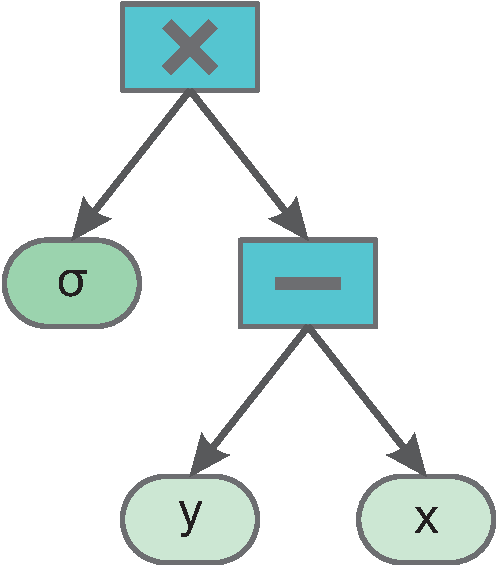
\includegraphics[draft=false,scale=0.24]{lorenz_expressions_eq1.pdf} \hspace{1ex} } 
\raisebox{1ex-\height}{ 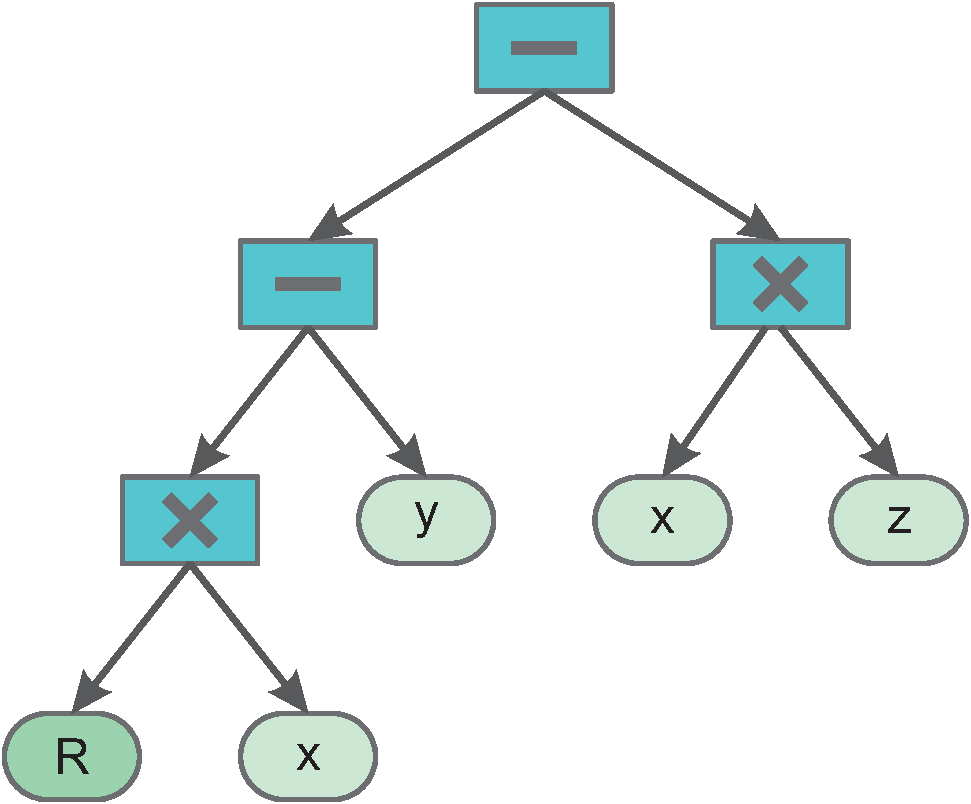
\includegraphics[draft=false,scale=0.24]{lorenz_expressions_eq2.pdf} \hspace{1ex} } 
\raisebox{1ex-\height}{ 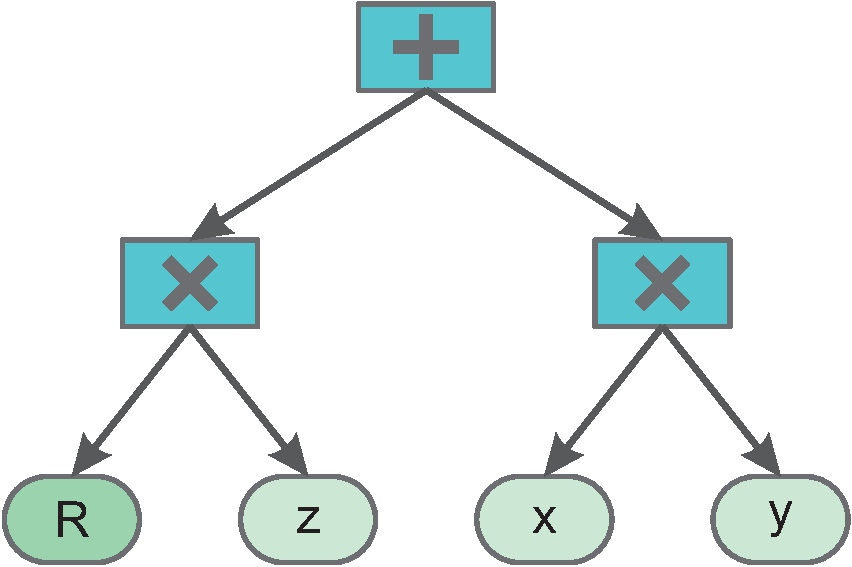
\includegraphics[draft=false,scale=0.24]{lorenz_expressions_eq3.pdf} }

\end{frame}




\begin{frame}[fragile]{The algorithm -- Evaluation of the expression tree}

Recursive determination of the Taylor coefficients
\begin{itemize}
 \item[1.] Initialize $X_0 = x(t)$ 
 \item[2.] Calculate $X_1 = F_0( X_0 )$ 
 \item[3.] Calculate $X_2 = \frac{1}{2} F_1( X_0 , X_1 )$ 
 \item[4.] Calculate $X_3 = \frac{1}{3} F_2( X_0 , X_1 , X_2 )$
 \item[\dots]
 \item[ ] Calculate $X_s = \frac{1}{s} F_{s-1}( X_0 , X_1 , \dots , X_{s-1} )$
 \item[ ]
 \item[ ] Finally $x(t+\Delta t ) = X_0 + \Delta t X_1 + \Delta t^2 X_2 + \dots $
\end{itemize}

\vspace{4ex}

\pause

{\bf In every iteration the expression tree is evaluated!}


\end{frame}




\begin{frame}[fragile]{Algebraic operations}

At every iteration the nodes in the expression tree have to be evaluated

\vspace{2ex}
Formulas for iteration $i$:

\begin{itemize}
 \item Constants: $C_i = c \delta_{i,0}$
 \item Dependend variable $x$: $X_i$
 \item Summation $s=l+r$: $S_i = L_i + R_i$
 \item Multiplication $m=l \times r$: $M_i = \sum\limits_{j=0}^i L_j R_{i-j}$
 \item Division $d=l/r$: $D_i = 1 / R_0 ( L_i - \sum\limits_{j=0}^{i-1} D_j R_{i-j} )$
 \item Formulas for special functions exist: $\exp$, $\log$, $\cos$, $\sin$, \dots
\end{itemize}

\end{frame}






\begin{frame}[fragile]{Algebraic operations -- Formulas}

At every iteration the nodes in the expression tree have to be evaluated. Formulas for iteration $i$:

\vspace{1ex}

{\small
\begin{tabular}{m{0.1\textwidth}@{\hspace{0.05\textwidth}}m{0.35\textwidth}@{\hspace{0.05\textwidth}}m{0.4\textwidth}}
 \vspace{0.1ex}\hspace{2ex}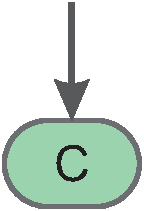
\includegraphics[draft=false,scale=0.2]{nodes_constant.pdf} & Constants: & $C_i = c \delta_{i,0}$ \\
 \hline
 \vspace{0.6ex}\hspace{2ex}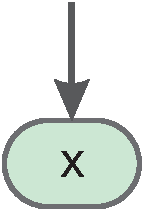
\includegraphics[draft=false,scale=0.2]{nodes_variable.pdf} & Dependend variable: $x$ & $X_i$ \\
 \hline
 \vspace{0.6ex}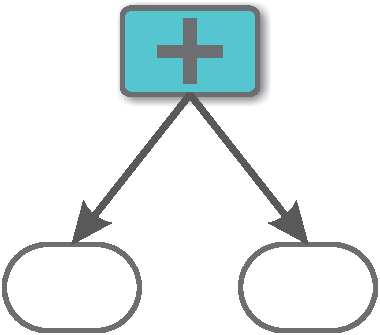
\includegraphics[draft=false,scale=0.2]{nodes_plus.pdf} &  Summation $s=l+r$: & $S_i = L_i + R_i$ \\
 \hline
 \vspace{0.6ex}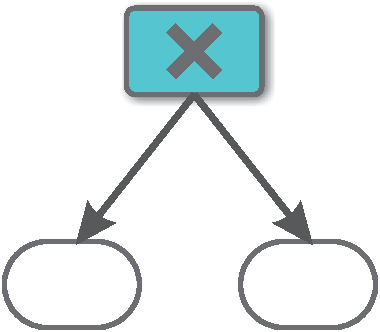
\includegraphics[draft=false,scale=0.2]{nodes_multiplies.pdf} & Multiplication $m=l \times r$: & $M_i = \sum\limits_{j=0}^i L_j R_{i-j}$ \\
 \hline
 \vspace{0.6ex}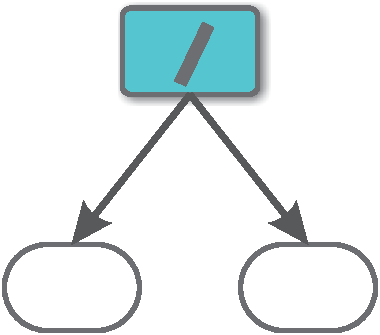
\includegraphics[draft=false,scale=0.2]{nodes_divides.pdf} & Division $d=l/r$: & $D_i = 1 / R_0 ( L_i - \sum\limits_{j=0}^{i-1} D_j R_{i-j} )$ \\
 \hline
 \vspace{0.6ex}\hspace{2ex}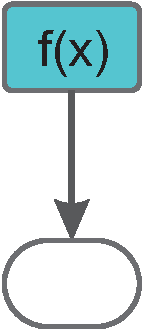
\includegraphics[draft=false,scale=0.2]{nodes_function.pdf} & Formulas for special functions exist & 
\end{tabular}}

\end{frame}








\begin{frame}[fragile]{Nice side effects}

Step size control
\begin{itemize}
 \item Error estimate: $err = X_s$
 \item $v = || \frac{err_k}{\epsilon_{rel} + \epsilon_{abs} |x_k| } ||$
 \item $\Delta t = v^{-1/s}$
 \item No acceptance or rejection step is required
\end{itemize}

\vspace{2ex}
Dense output is trivially present
\begin{itemize}
 \item $x(t+\tau) = X_0 + \tau X_1 + \tau^2 X_2 + \tau^3 X_3 + \dots $, \hspace{4ex} $0 < \tau < \Delta t$
\end{itemize}

\vspace{2ex}
Methods for order estimation exist


 

\end{frame}





\section{Implementation}



\frame{\tableofcontents[currentsection]}





\begin{frame}[fragile]{Implementation}

\centerline{\Large \bf \color{red}Taylor}

\vspace{2ex}

Download
\begin{itemize}
\item \texttt{https://github.com/headmyshoulder/taylor}
\end{itemize}

\pause

\vspace{2ex}

Taylor will be integrated into {\bf odeint}

\begin{itemize}
 \item Implements some odeint - stepper
\end{itemize}

\pause

\vspace{2ex}

Modern C++
\begin{itemize}
 \item Heavy use of the C++ template systems
 \item Expression templates for expression trees
 \item Template meta-programming 
\end{itemize}


\end{frame}








\begin{frame}{C++ Templates}
 \begin{itemize}
  \item Here, C++ templates will be used to create the expression tree -- \textbf{Expression Templates}
  \item Template Metaprogramming to evaluate the expression templates
  \item It basically means using the template engine to generate a program from which the compiler creates then the binary
        \item C++ compilers always use the template engine (no additional compile step required)
 \end{itemize}

 \pause

 \begin{itemize}
         \item Template engine and templates are a functional programming language
         \item Templates form a Turing-complete programming language
         \item $\longrightarrow$ You can solve any problem with the template engine
 \end{itemize}

\end{frame}






\begin{frame}[fragile]{Expression templates}

\begin{lstlisting}{language=c++}
template< class L , class R > struct binary_expression
{
    binary_expression( string name , L l , R r )
    ... 
    L m_l;
    R m_r;
};

struct terminal_expression
{
    terminal_expression( string name ) ...
};

const terminal_expression arg1( "arg1" ) , arg2( "arg2" );

template< class L , class R >
binary_expression< L , R > operator+( L l , R r )
{
    return binary_expression< L , R >( "Plus" , l , r );
}
...

template< class Expr > void print( Expr expr ) { ... }

print( arg1 );
print( arg1 + ( arg2 + arg1 - arg2 ) );
\end{lstlisting}



\end{frame}

\begin{frame}[fragile]{Expression templates}

\begin{itemize}
  \item Expression template are constructed during compile-time
  \item Strong optimization -- no performance loss
  \item Lazyness
  \item Applications: Linear algebra systems, AD, (E)DSL
\end{itemize}

\vspace{2ex}
Example MTL4
 \begin{lstlisting}{language=c++}
   mtl4::dense_matrix< double > m1( n , n ) , m2( n , n ) , m3( n , n ) ;
   
   // do something useful with m1, m2, m3
   
   mtl4::dense_matrix< double > result = m1 + 5.0 * m2 + 0.5 * m3 ;
 \end{lstlisting}

\vspace{2ex}
Last line creates an expression template which is evaluated to
\begin{lstlisting}{language=c++}
 for( int i=0 ; i<n ; ++i )
    for( int j=0 ; j<n ; ++j )
       result( i , j ) = m1( i , j ) + 5.0 * m2( i , j ) + 0.5 * m3( i , j );
\end{lstlisting}

\end{frame}








\begin{frame}[fragile]{First example -- Lorenz system}

\begin{lstlisting}{language=c++}
taylor_direct_fixed_order< 25 , 3 > stepper;
state_type x = {{ 10.0 , 10.0 , 10.0 }} ;
double t = 0.0;
double dt = 1.0;
while( t < 50000.0 )
{
    stepper.try_step(
        fusion::make_vector(
            sigma * ( arg2 - arg1 ) ,
            R * arg1 - arg2 - arg1 * arg3 ,
            arg1 * arg2 - b * arg3
            ) , x , t , dt );
    cout << t << "\t" << x << "\t" << dt << endl;
}
\end{lstlisting}

\begin{itemize}
 \item ODE is a compile time sequence of expression templates
 \item The expression template is defined with {\tt boost::proto}
 \item {\bf No preprocessing step is necessary!}
\end{itemize}


\end{frame}


\begin{frame}[fragile]{Expression templates and ODEs}
 
Boost.Proto (C++ library)
\begin{itemize}
  \item Creation, manipulation and evaluation of the syntax tree
  \item Grammar = Allowed expression + (optional) Transformation
\end{itemize}

\vspace{2ex}

\pause

Taylor library uses Proto as front end:
\begin{itemize}
  \item The ODE is a set of Proto expression templates
  \item ODE is transformed into a custom expression template
\end{itemize}

\vspace{2ex}

\begin{lstlisting}{language=c++}
struct tree_generator :
    proto::or_
    <
        variable_generator< proto::_ > ,
        constant_generator ,
        plus_generator< tree_generator > ,
        minus_generator< tree_generator > ,
        multiplies_generator< tree_generator > ,
        divides_generator< tree_generator > ,
        unary_generator< tree_generator >
    > { };
\end{lstlisting}

\end{frame}

\begin{frame}[fragile]{Expression templates and ODEs}

\begin{itemize}
  \item Evaluation of the custom template -- iteration several times of the template
  \item The nodes implement the rules for the algebraic expressions
  \item Optimzation of the expression tree \hspace{2ex} \raisebox{1ex-\height}{ 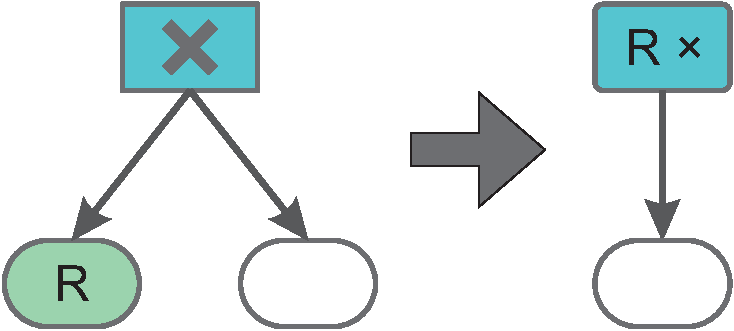
\includegraphics[draft=false,scale=0.25]{node_transformation.pdf} }
\end{itemize}

\vspace{2ex}

Example: The plus node
\begin{lstlisting}{language=c++}
template< class Left , class Right >
struct plus_node : binary_node< Left , Right >
{
    plus_node( const Left &left , const Right &right )
    : binary_node< Left , Right >( left , right ) { }

    template< class State , class Derivs >
    Value operator()( const State &x , const Derivs &derivs , size_t which )
    {
        return m_left( x , derivs , which ) + m_right( x , derivs , which );
    }
};
\end{lstlisting}
 
\end{frame}

\begin{frame}[fragile]{The interface}

Interface for easy implementation of arbitrary ODEs exist
\begin{lstlisting}{language=c++}
taylor_direct_fixed_order< 25 , 3 > stepper;
stepper.try_step( sys , x , t , dt );
\end{lstlisting}

\vspace{1ex}
{\tt sys} represents the ODE, Example:
\begin{lstlisting}{language=c++}
fusion::make_vector(
            sigma * ( arg2 - arg1 ) ,
            R * arg1 - arg2 - arg1 * arg3 ,
            arg1 * arg2 - b * arg3 )
 \end{lstlisting}


\vspace{1ex}
{\tt x} is the state of the ODE is in-place transformed

\vspace{1ex}
{\tt t,dt} are the time and the step size

\end{frame}





\begin{frame}[fragile]{Results}

Performance comparison against full Fortran code

\begin{itemize}
 \item The Lorenz system as test system
 \item Benchmarking: a Fortran code with a non-AD implementation
 \item Both codes have the same performance, run-time deviation is less 20\%
 \item Exact result depends strongly on the used compiler (gcc 4.5, gcc 4.6, gfortran, ...)
\end{itemize}

\end{frame}



\begin{frame}[fragile]{Comparison against other mehtods}

\centerline{
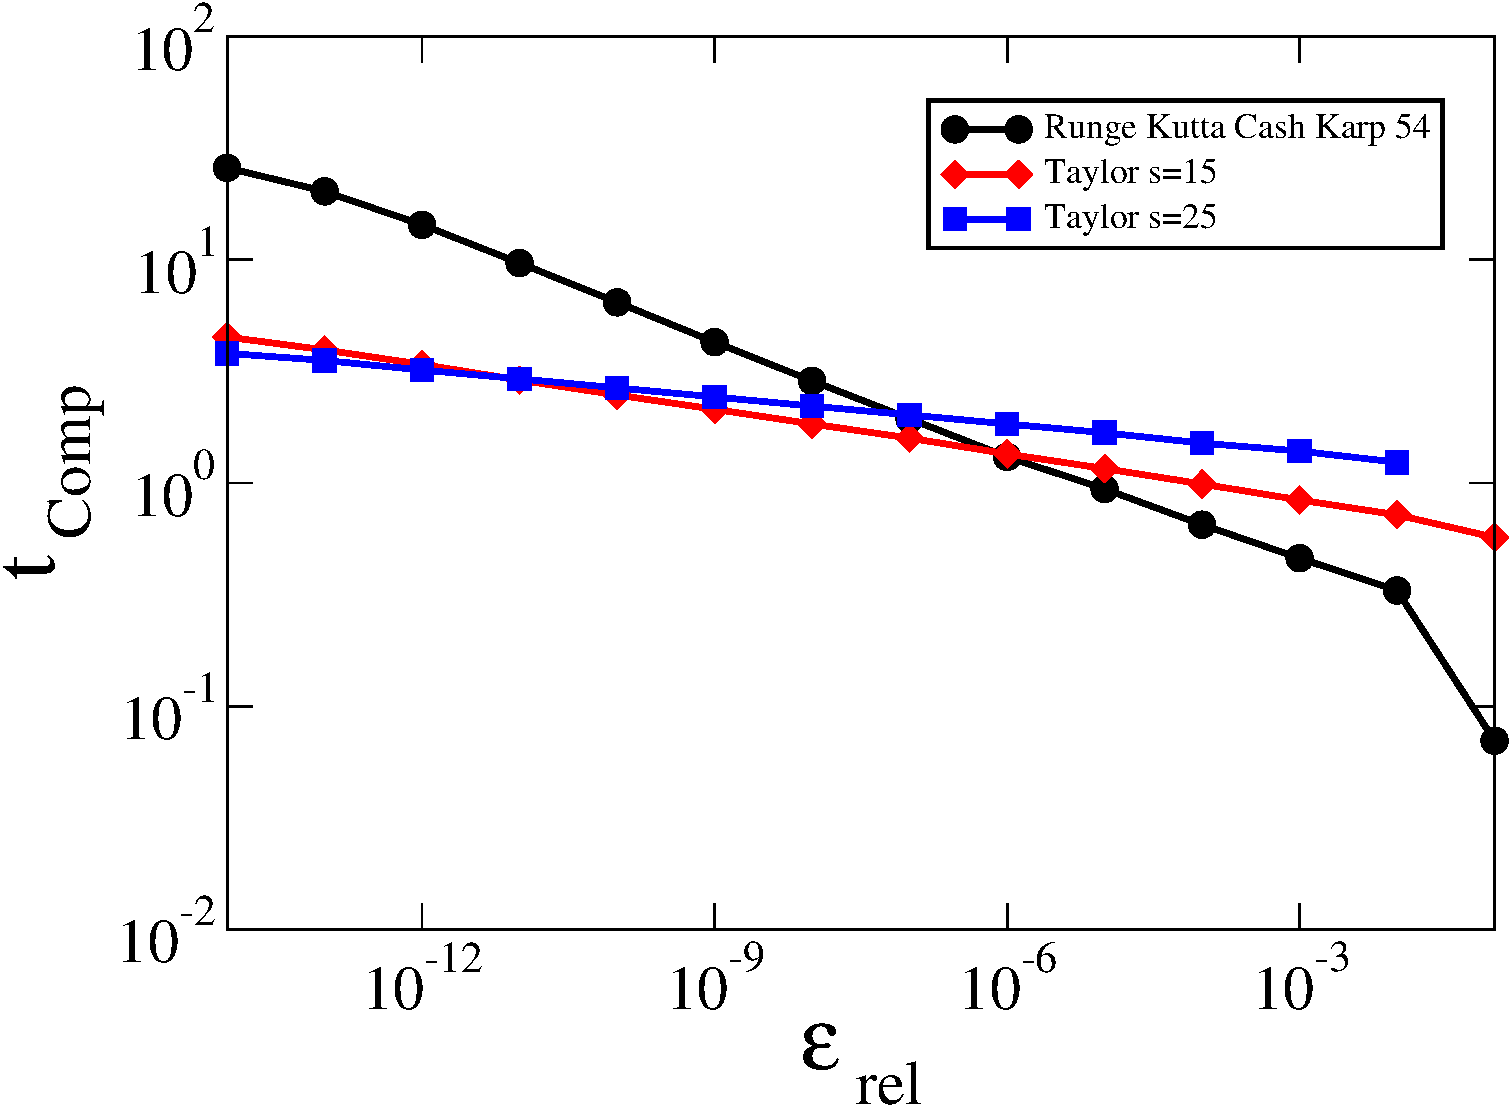
\includegraphics[draft=false,width=0.5\textwidth]{stepper_comp.pdf}
}

\begin{itemize}
 \item Taylor has good performance for high precision
 \item Outperforms the classical Runge-Kutta steppers
\end{itemize}


\end{frame}




\section{Conclusion}

\begin{frame}[fragile]{Conclusion}

  \begin{itemize}
    \item Taylor -- A C++ library for the Taylor series method of ordinary differential equations
    \item Uses expression templates as basis for the automatic differentiation
    \item Fast
    \item Uses modern C++ methods
    \item Template Metaprogramming is the main programming technique
  \end{itemize}

\end{frame}


\begin{frame}[fragile]{Outlook}

The library is not complete
\begin{itemize}
 \item Implementation of special functions
 \item Implementation of stencils for lattice equations
 \item Implementation of variable order
 \item Implementation of dense output functionality
 \item Portability layer for arbitrary precision types
 \item Integration into odeint
\end{itemize}

\end{frame}


\begin{frame}[fragile]{Resources}

Download and development

{\tt https://www.github.com/headmyshoulder/taylor}

\vspace{2ex}

Odeint 

{\tt odeint.com}

\vspace{4ex}

\begin{block}{Contributions and feedback}
 are highly welcome
\end{block}

\end{frame}



\end{document}
